\documentclass{beamer}
\usetheme{metropolis}

\usepackage[utf8]{inputenc}
\usepackage{epiolmec}

\title{Buenos tipos para el desarrollo web}
\date{29 de febrero de 2016}
\author{Alejandro Serrano}
\institute{Haskell-MAD}

%% ODER: format ==         = "\mathrel{==}"
%% ODER: format /=         = "\neq "
%
%
\makeatletter
\@ifundefined{lhs2tex.lhs2tex.sty.read}%
  {\@namedef{lhs2tex.lhs2tex.sty.read}{}%
   \newcommand\SkipToFmtEnd{}%
   \newcommand\EndFmtInput{}%
   \long\def\SkipToFmtEnd#1\EndFmtInput{}%
  }\SkipToFmtEnd

\newcommand\ReadOnlyOnce[1]{\@ifundefined{#1}{\@namedef{#1}{}}\SkipToFmtEnd}
\usepackage{amstext}
\usepackage{amssymb}
\usepackage{stmaryrd}
\DeclareFontFamily{OT1}{cmtex}{}
\DeclareFontShape{OT1}{cmtex}{m}{n}
  {<5><6><7><8>cmtex8
   <9>cmtex9
   <10><10.95><12><14.4><17.28><20.74><24.88>cmtex10}{}
\DeclareFontShape{OT1}{cmtex}{m}{it}
  {<-> ssub * cmtt/m/it}{}
\newcommand{\texfamily}{\fontfamily{cmtex}\selectfont}
\DeclareFontShape{OT1}{cmtt}{bx}{n}
  {<5><6><7><8>cmtt8
   <9>cmbtt9
   <10><10.95><12><14.4><17.28><20.74><24.88>cmbtt10}{}
\DeclareFontShape{OT1}{cmtex}{bx}{n}
  {<-> ssub * cmtt/bx/n}{}
\newcommand{\tex}[1]{\text{\texfamily#1}}	% NEU

\newcommand{\Sp}{\hskip.33334em\relax}


\newcommand{\Conid}[1]{\mathit{#1}}
\newcommand{\Varid}[1]{\mathit{#1}}
\newcommand{\anonymous}{\kern0.06em \vbox{\hrule\@width.5em}}
\newcommand{\plus}{\mathbin{+\!\!\!+}}
\newcommand{\bind}{\mathbin{>\!\!\!>\mkern-6.7mu=}}
\newcommand{\rbind}{\mathbin{=\mkern-6.7mu<\!\!\!<}}% suggested by Neil Mitchell
\newcommand{\sequ}{\mathbin{>\!\!\!>}}
\renewcommand{\leq}{\leqslant}
\renewcommand{\geq}{\geqslant}
\usepackage{polytable}

%mathindent has to be defined
\@ifundefined{mathindent}%
  {\newdimen\mathindent\mathindent\leftmargini}%
  {}%

\def\resethooks{%
  \global\let\SaveRestoreHook\empty
  \global\let\ColumnHook\empty}
\newcommand*{\savecolumns}[1][default]%
  {\g@addto@macro\SaveRestoreHook{\savecolumns[#1]}}
\newcommand*{\restorecolumns}[1][default]%
  {\g@addto@macro\SaveRestoreHook{\restorecolumns[#1]}}
\newcommand*{\aligncolumn}[2]%
  {\g@addto@macro\ColumnHook{\column{#1}{#2}}}

\resethooks

\newcommand{\onelinecommentchars}{\quad-{}- }
\newcommand{\commentbeginchars}{\enskip\{-}
\newcommand{\commentendchars}{-\}\enskip}

\newcommand{\visiblecomments}{%
  \let\onelinecomment=\onelinecommentchars
  \let\commentbegin=\commentbeginchars
  \let\commentend=\commentendchars}

\newcommand{\invisiblecomments}{%
  \let\onelinecomment=\empty
  \let\commentbegin=\empty
  \let\commentend=\empty}

\visiblecomments

\newlength{\blanklineskip}
\setlength{\blanklineskip}{0.66084ex}

\newcommand{\hsindent}[1]{\quad}% default is fixed indentation
\let\hspre\empty
\let\hspost\empty
\newcommand{\NB}{\textbf{NB}}
\newcommand{\Todo}[1]{$\langle$\textbf{To do:}~#1$\rangle$}

\EndFmtInput
\makeatother
%
%
%
%
%
%
% This package provides two environments suitable to take the place
% of hscode, called "plainhscode" and "arrayhscode". 
%
% The plain environment surrounds each code block by vertical space,
% and it uses \abovedisplayskip and \belowdisplayskip to get spacing
% similar to formulas. Note that if these dimensions are changed,
% the spacing around displayed math formulas changes as well.
% All code is indented using \leftskip.
%
% Changed 19.08.2004 to reflect changes in colorcode. Should work with
% CodeGroup.sty.
%
\ReadOnlyOnce{polycode.fmt}%
\makeatletter

\newcommand{\hsnewpar}[1]%
  {{\parskip=0pt\parindent=0pt\par\vskip #1\noindent}}

% can be used, for instance, to redefine the code size, by setting the
% command to \small or something alike
\newcommand{\hscodestyle}{}

% The command \sethscode can be used to switch the code formatting
% behaviour by mapping the hscode environment in the subst directive
% to a new LaTeX environment.

\newcommand{\sethscode}[1]%
  {\expandafter\let\expandafter\hscode\csname #1\endcsname
   \expandafter\let\expandafter\endhscode\csname end#1\endcsname}

% "compatibility" mode restores the non-polycode.fmt layout.

\newenvironment{compathscode}%
  {\par\noindent
   \advance\leftskip\mathindent
   \hscodestyle
   \let\\=\@normalcr
   \let\hspre\(\let\hspost\)%
   \pboxed}%
  {\endpboxed\)%
   \par\noindent
   \ignorespacesafterend}

\newcommand{\compaths}{\sethscode{compathscode}}

% "plain" mode is the proposed default.
% It should now work with \centering.
% This required some changes. The old version
% is still available for reference as oldplainhscode.

\newenvironment{plainhscode}%
  {\hsnewpar\abovedisplayskip
   \advance\leftskip\mathindent
   \hscodestyle
   \let\hspre\(\let\hspost\)%
   \pboxed}%
  {\endpboxed%
   \hsnewpar\belowdisplayskip
   \ignorespacesafterend}

\newenvironment{oldplainhscode}%
  {\hsnewpar\abovedisplayskip
   \advance\leftskip\mathindent
   \hscodestyle
   \let\\=\@normalcr
   \(\pboxed}%
  {\endpboxed\)%
   \hsnewpar\belowdisplayskip
   \ignorespacesafterend}

% Here, we make plainhscode the default environment.

\newcommand{\plainhs}{\sethscode{plainhscode}}
\newcommand{\oldplainhs}{\sethscode{oldplainhscode}}
\plainhs

% The arrayhscode is like plain, but makes use of polytable's
% parray environment which disallows page breaks in code blocks.

\newenvironment{arrayhscode}%
  {\hsnewpar\abovedisplayskip
   \advance\leftskip\mathindent
   \hscodestyle
   \let\\=\@normalcr
   \(\parray}%
  {\endparray\)%
   \hsnewpar\belowdisplayskip
   \ignorespacesafterend}

\newcommand{\arrayhs}{\sethscode{arrayhscode}}

% The mathhscode environment also makes use of polytable's parray 
% environment. It is supposed to be used only inside math mode 
% (I used it to typeset the type rules in my thesis).

\newenvironment{mathhscode}%
  {\parray}{\endparray}

\newcommand{\mathhs}{\sethscode{mathhscode}}

% texths is similar to mathhs, but works in text mode.

\newenvironment{texthscode}%
  {\(\parray}{\endparray\)}

\newcommand{\texths}{\sethscode{texthscode}}

% The framed environment places code in a framed box.

\def\codeframewidth{\arrayrulewidth}
\RequirePackage{calc}

\newenvironment{framedhscode}%
  {\parskip=\abovedisplayskip\par\noindent
   \hscodestyle
   \arrayrulewidth=\codeframewidth
   \tabular{@{}|p{\linewidth-2\arraycolsep-2\arrayrulewidth-2pt}|@{}}%
   \hline\framedhslinecorrect\\{-1.5ex}%
   \let\endoflinesave=\\
   \let\\=\@normalcr
   \(\pboxed}%
  {\endpboxed\)%
   \framedhslinecorrect\endoflinesave{.5ex}\hline
   \endtabular
   \parskip=\belowdisplayskip\par\noindent
   \ignorespacesafterend}

\newcommand{\framedhslinecorrect}[2]%
  {#1[#2]}

\newcommand{\framedhs}{\sethscode{framedhscode}}

% The inlinehscode environment is an experimental environment
% that can be used to typeset displayed code inline.

\newenvironment{inlinehscode}%
  {\(\def\column##1##2{}%
   \let\>\undefined\let\<\undefined\let\\\undefined
   \newcommand\>[1][]{}\newcommand\<[1][]{}\newcommand\\[1][]{}%
   \def\fromto##1##2##3{##3}%
   \def\nextline{}}{\) }%

\newcommand{\inlinehs}{\sethscode{inlinehscode}}

% The joincode environment is a separate environment that
% can be used to surround and thereby connect multiple code
% blocks.

\newenvironment{joincode}%
  {\let\orighscode=\hscode
   \let\origendhscode=\endhscode
   \def\endhscode{\def\hscode{\endgroup\def\@currenvir{hscode}\\}\begingroup}
   %\let\SaveRestoreHook=\empty
   %\let\ColumnHook=\empty
   %\let\resethooks=\empty
   \orighscode\def\hscode{\endgroup\def\@currenvir{hscode}}}%
  {\origendhscode
   \global\let\hscode=\orighscode
   \global\let\endhscode=\origendhscode}%

\makeatother
\EndFmtInput
%


\begin{document}
\maketitle

\section{¿De qué va esta charla?}

\section{Una pausa para la publicidad}

\begin{frame}[fragile]
\frametitle{Hola, me llamo Alejandro}
\begin{columns}
\column{0.55\textwidth}
\begin{itemize}
\item Nací y he crecido en Madrid
\item Comencé a interesarme por Haskell allá por el 2009
\item He participado dos veces en el Google Summer of Code mejorando el soporte de Haskell para Eclipse y Emacs
\item El año pasado publiqué un libro, \emph{Beginning Haskell}
\end{itemize}
\column{0.45\textwidth}

\includegraphics[scale=0.2]{libro.jpg}
\end{columns}
\end{frame}

\begin{frame}[fragile]
\frametitle{Vivo en Utrecht (Países Bajos)}
\begin{columns}
\column{0.45\textwidth}
\begin{itemize}
\item En la Universidad tienen un grupo especializado en prog. funcional
\item Me fui de Erasmus en 2010/11 para aprender
\item Y ahora vivo allí y me estoy doctorando :)
\end{itemize}
\column{0.55\textwidth}
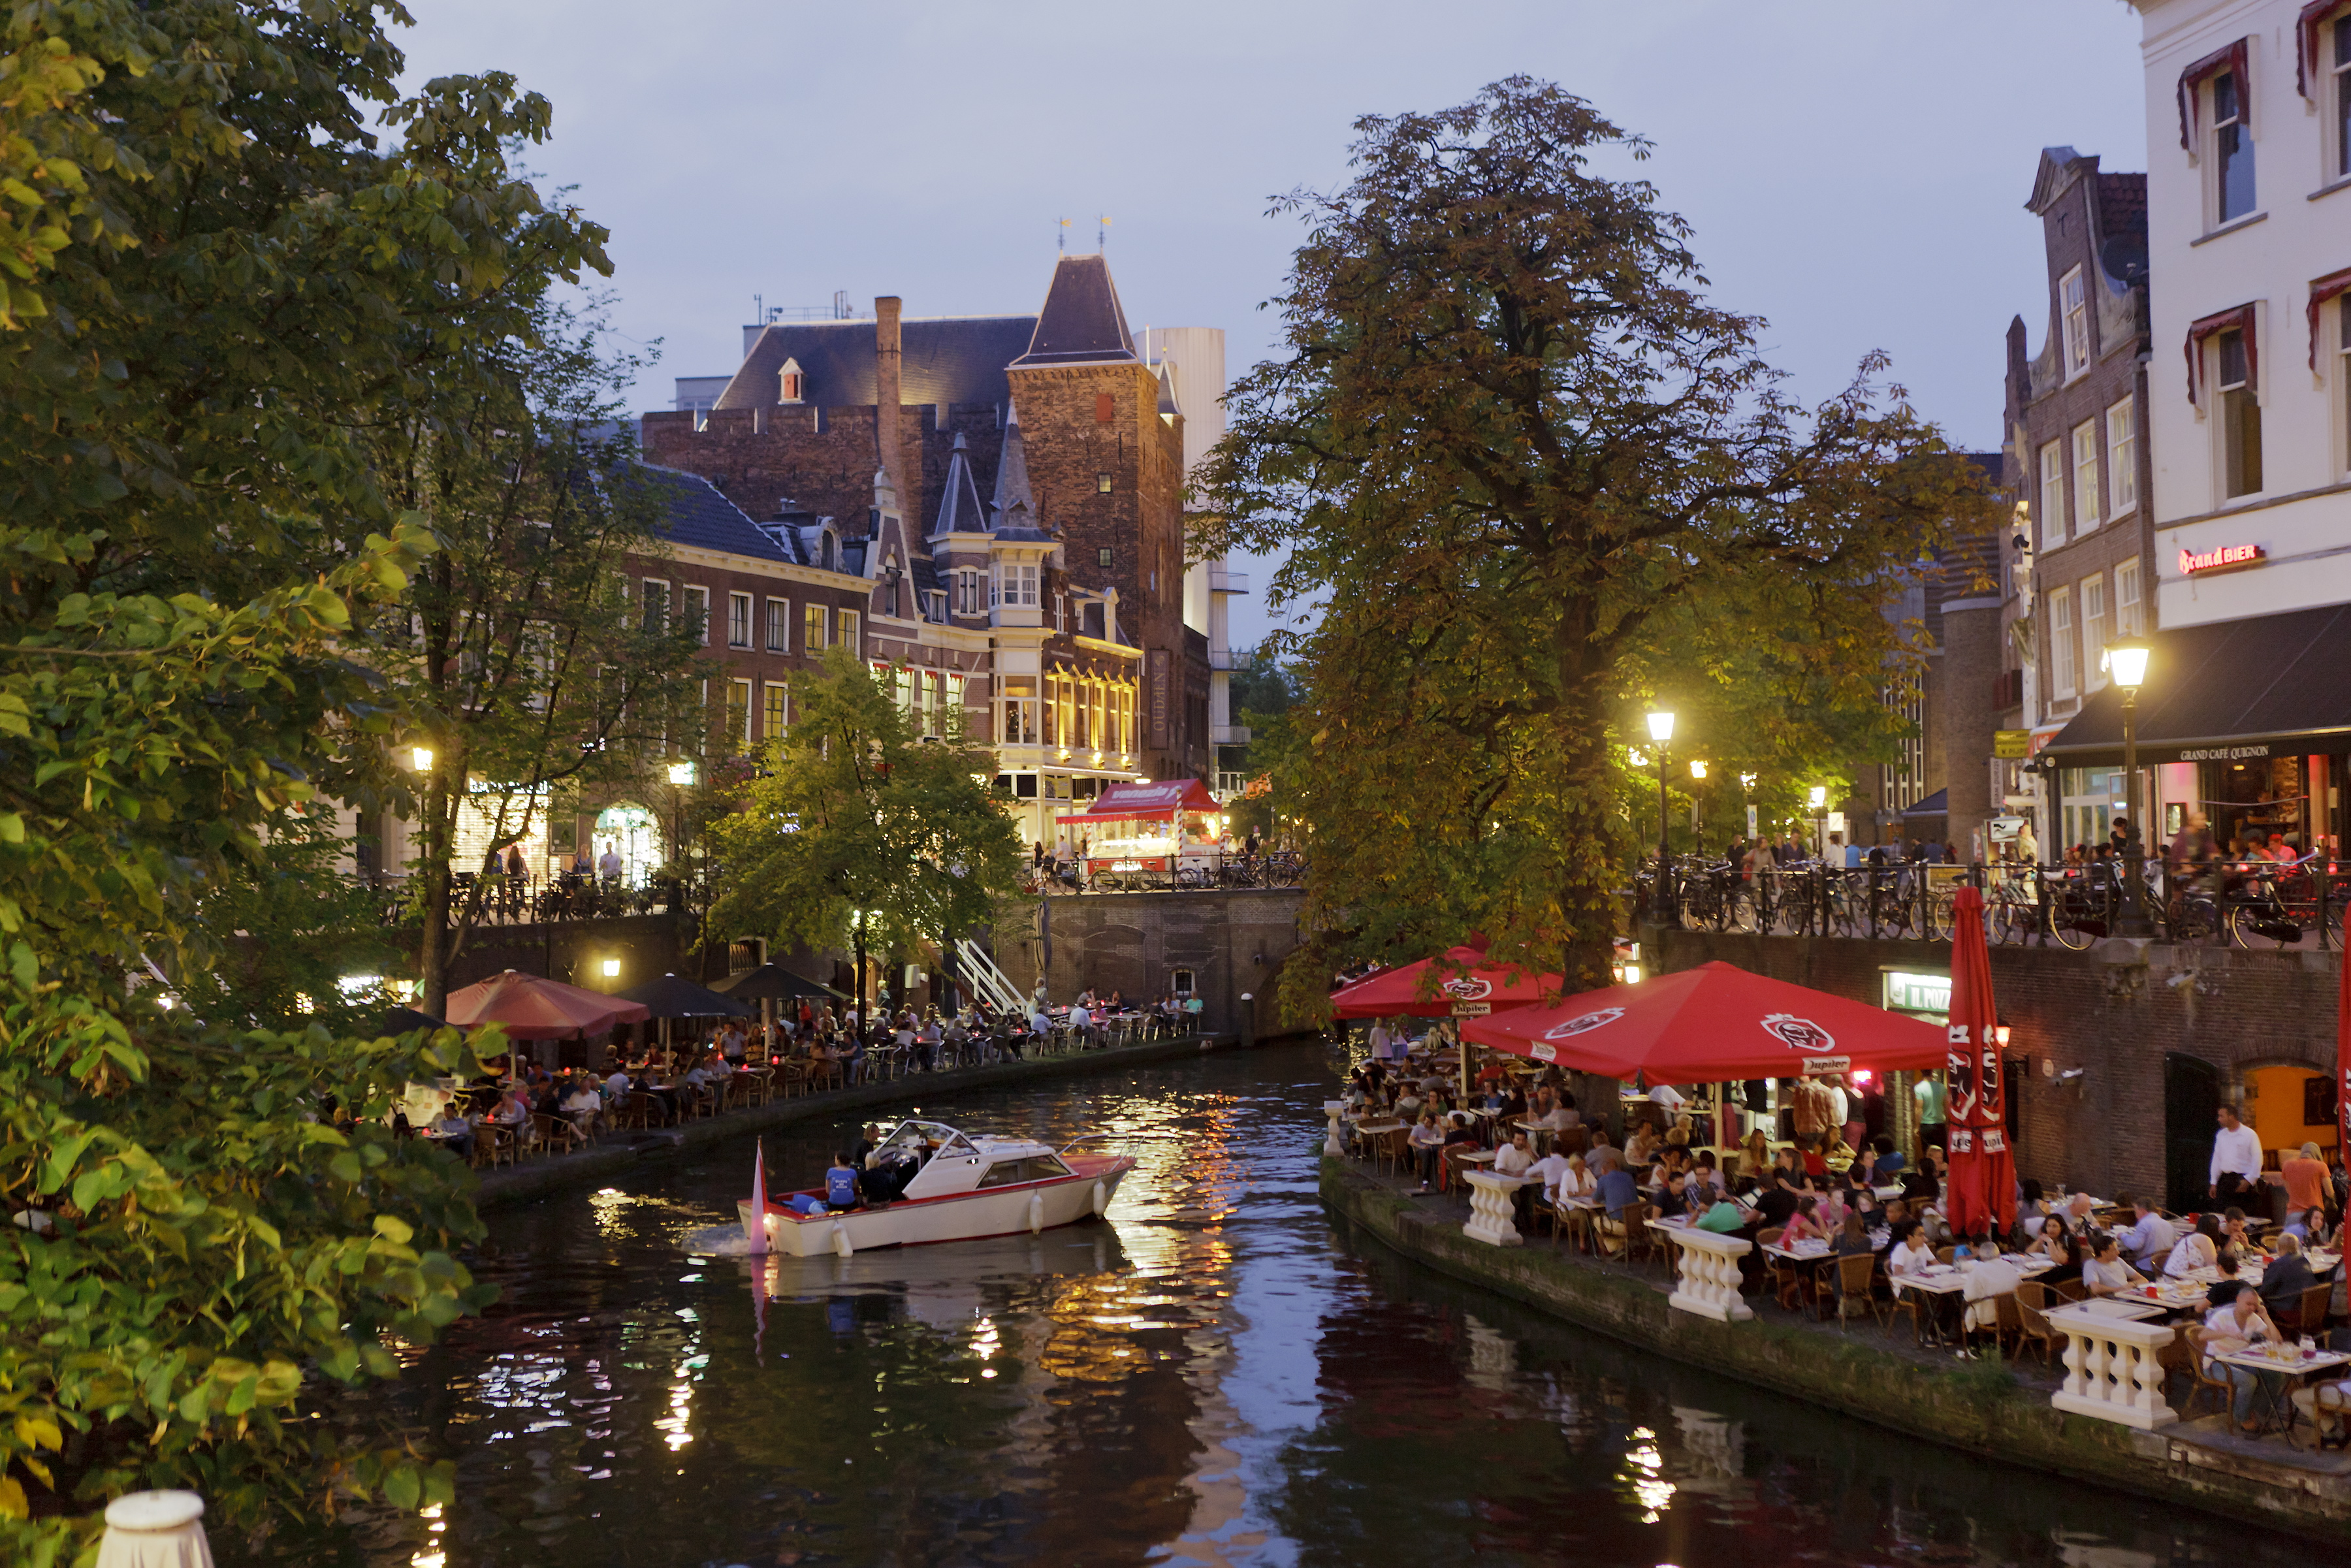
\includegraphics[scale=0.2]{utrecht.jpg}
\end{columns}
\

Todos los veranos organizamos un curso de 2 semanas: \\
\emph{\Large Applied Functional Programming} \\
(este año es del 4 al 15 de julio)
\end{frame}

\section{Jugando con tipos (sin quemarnos)}

%1
\begin{frame}[fragile]
\frametitle{Tipos de datos algebraicos}
\begin{hscode}\SaveRestoreHook
\column{B}{@{}>{\hspre}l<{\hspost}@{}}%
\column{15}{@{}>{\hspre}c<{\hspost}@{}}%
\column{15E}{@{}l@{}}%
\column{18}{@{}>{\hspre}l<{\hspost}@{}}%
\column{E}{@{}>{\hspre}l<{\hspost}@{}}%
\>[B]{}\mathbf{data}\;\Conid{Numero}{}\<[15]%
\>[15]{}\mathrel{=}{}\<[15E]%
\>[18]{}\Conid{Cero}{}\<[E]%
\\
\>[15]{}\mid {}\<[15E]%
\>[18]{}\Conid{Suc}\;\Conid{Numero}{}\<[E]%
\\[\blanklineskip]%
\>[B]{}\mathbf{data}\;\Conid{Arbol}\;\Varid{a}{}\<[15]%
\>[15]{}\mathrel{=}{}\<[15E]%
\>[18]{}\Conid{Hoja}\;\Varid{a}{}\<[E]%
\\
\>[15]{}\mid {}\<[15E]%
\>[18]{}\Conid{Nodo}\;(\Conid{Arbol}\;\Varid{a})\;\Varid{a}\;(\Conid{Arbol}\;\Varid{a}){}\<[E]%
\ColumnHook
\end{hscode}\resethooks
\begin{tabbing}\tt
~\char42{}Charla\char62{}~\char58{}t~Suc~\char40{}Suc~Cero\char41{}\\
\tt ~Suc~\char40{}Suc~Cero\char41{}~\char58{}\char58{}~Numero\\
\tt ~\char42{}Charla\char62{}~\char58{}t~Nodo~\char40{}Hoja~\char39{}a\char39{}\char41{}~\char39{}b\char39{}~\char40{}Hoja~\char39{}c\char39{}\char41{}\\
\tt ~Nodo~\char40{}Hoja~\char39{}a\char39{}\char41{}~\char39{}b\char39{}~\char40{}Hoja~\char39{}c\char39{}\char41{}~\char58{}\char58{}~Arbol~Char
\end{tabbing}
\end{frame}

%2
\begin{frame}[fragile]
\frametitle{Declarando el tipo de los constructores}
\begin{hscode}\SaveRestoreHook
\column{B}{@{}>{\hspre}l<{\hspost}@{}}%
\column{15}{@{}>{\hspre}c<{\hspost}@{}}%
\column{15E}{@{}l@{}}%
\column{18}{@{}>{\hspre}l<{\hspost}@{}}%
\column{26}{@{}>{\hspre}l<{\hspost}@{}}%
\column{28}{@{}>{\hspre}l<{\hspost}@{}}%
\column{E}{@{}>{\hspre}l<{\hspost}@{}}%
\>[B]{}\mathbf{data}\;\Conid{Numero}{}\<[15]%
\>[15]{}\mathrel{=}{}\<[15E]%
\>[18]{}\Conid{Cero}\mid {}\<[26]%
\>[26]{}\Conid{Suc}\;\Conid{Numero}{}\<[E]%
\\[\blanklineskip]%
\>[B]{}\mathbf{data}\;\Conid{Arbol}\;\Varid{a}{}\<[15]%
\>[15]{}\mathrel{=}{}\<[15E]%
\>[18]{}\Conid{Hoja}\;\Varid{a}\mid {}\<[28]%
\>[28]{}\Conid{Nodo}\;(\Conid{Arbol}\;\Varid{a})\;\Varid{a}\;(\Conid{Arbol}\;\Varid{a}){}\<[E]%
\ColumnHook
\end{hscode}\resethooks
\begin{hscode}\SaveRestoreHook
\column{B}{@{}>{\hspre}l<{\hspost}@{}}%
\column{3}{@{}>{\hspre}l<{\hspost}@{}}%
\column{9}{@{}>{\hspre}l<{\hspost}@{}}%
\column{23}{@{}>{\hspre}l<{\hspost}@{}}%
\column{37}{@{}>{\hspre}l<{\hspost}@{}}%
\column{E}{@{}>{\hspre}l<{\hspost}@{}}%
\>[B]{}\mbox{\enskip\{-\# LANGUAGE GADTs  \#-\}\enskip}{}\<[E]%
\\[\blanklineskip]%
\>[B]{}\mathbf{data}\;\Conid{Numero}\;\mathbf{where}{}\<[E]%
\\
\>[B]{}\hsindent{3}{}\<[3]%
\>[3]{}\Conid{Cero}{}\<[9]%
\>[9]{}\mathbin{::}{}\<[23]%
\>[23]{}\Conid{Numero}{}\<[E]%
\\
\>[B]{}\hsindent{3}{}\<[3]%
\>[3]{}\Conid{Suc}{}\<[9]%
\>[9]{}\mathbin{::}\Conid{Numero}\to {}\<[23]%
\>[23]{}\Conid{Numero}{}\<[E]%
\\[\blanklineskip]%
\>[B]{}\mathbf{data}\;\Conid{Arbol}\;\Varid{a}\;\mathbf{where}{}\<[E]%
\\
\>[B]{}\hsindent{3}{}\<[3]%
\>[3]{}\Conid{Hoja}{}\<[9]%
\>[9]{}\mathbin{::}\Varid{a}{}\<[37]%
\>[37]{}\to \Conid{Arbol}\;\Varid{a}{}\<[E]%
\\
\>[B]{}\hsindent{3}{}\<[3]%
\>[3]{}\Conid{Nodo}{}\<[9]%
\>[9]{}\mathbin{::}\Conid{Arbol}\;\Varid{a}\to \Varid{a}\to \Conid{Arbol}\;\Varid{a}{}\<[37]%
\>[37]{}\to \Conid{Arbol}\;\Varid{a}{}\<[E]%
\ColumnHook
\end{hscode}\resethooks
\end{frame}

%3
\begin{frame}[fragile]
\frametitle{Describiendo campos de una tabla}
\begin{hscode}\SaveRestoreHook
\column{B}{@{}>{\hspre}l<{\hspost}@{}}%
\column{3}{@{}>{\hspre}l<{\hspost}@{}}%
\column{14}{@{}>{\hspre}l<{\hspost}@{}}%
\column{35}{@{}>{\hspre}l<{\hspost}@{}}%
\column{E}{@{}>{\hspre}l<{\hspost}@{}}%
\>[B]{}\mathbf{data}\;\Conid{CampoUsuario}\;\mathbf{where}{}\<[E]%
\\
\>[B]{}\hsindent{3}{}\<[3]%
\>[3]{}\Conid{Nombre}{}\<[14]%
\>[14]{}\mathbin{::}\Conid{String}{}\<[35]%
\>[35]{}\to \Conid{CampoUsuario}{}\<[E]%
\\
\>[B]{}\hsindent{3}{}\<[3]%
\>[3]{}\Conid{Apellidos}{}\<[14]%
\>[14]{}\mathbin{::}\Conid{String}{}\<[35]%
\>[35]{}\to \Conid{CampoUsuario}{}\<[E]%
\\
\>[B]{}\hsindent{3}{}\<[3]%
\>[3]{}\Conid{Edad}{}\<[14]%
\>[14]{}\mathbin{::}\Conid{Integer}{}\<[35]%
\>[35]{}\to \Conid{CampoUsuario}{}\<[E]%
\\
\>[B]{}\hsindent{3}{}\<[3]%
\>[3]{}\Conid{Direccion}{}\<[14]%
\>[14]{}\mathbin{::}\Conid{String}\to \Conid{String}{}\<[35]%
\>[35]{}\to \Conid{CampoUsuario}{}\<[E]%
\ColumnHook
\end{hscode}\resethooks

\pause
¿Qué tipo le damos a la siguiente función?
\vspace{-0.2cm}
\begin{tabbing}\tt
~\char42{}Charla\char62{}~getCampoUsuario~\char40{}Nombre~\char34{}Alejandro\char34{}\char41{}\\
\tt ~\char34{}Alejandro\char34{}~\char58{}\char58{}~String\\
\tt ~\char42{}Charla\char62{}~getCampoUsuario~\char40{}Edad~27\char41{}\\
\tt ~27~~~~~~~~~~\char58{}\char58{}~Integer
\end{tabbing}
\end{frame}

%4
\begin{frame}[fragile]
\frametitle{ADTs generalizados (GADTs)}
Los constructores pueden \emph{especializar} el tipo que construyen
\begin{hscode}\SaveRestoreHook
\column{B}{@{}>{\hspre}l<{\hspost}@{}}%
\column{3}{@{}>{\hspre}l<{\hspost}@{}}%
\column{14}{@{}>{\hspre}l<{\hspost}@{}}%
\column{35}{@{}>{\hspre}l<{\hspost}@{}}%
\column{E}{@{}>{\hspre}l<{\hspost}@{}}%
\>[B]{}\mathbf{data}\;\Conid{CampoUsuario}\;\Varid{a}\;\mathbf{where}{}\<[E]%
\\
\>[B]{}\hsindent{3}{}\<[3]%
\>[3]{}\Conid{Nombre}{}\<[14]%
\>[14]{}\mathbin{::}\Conid{String}{}\<[35]%
\>[35]{}\to \Conid{CampoUsuario}\;\Conid{String}{}\<[E]%
\\
\>[B]{}\hsindent{3}{}\<[3]%
\>[3]{}\Conid{Apellidos}{}\<[14]%
\>[14]{}\mathbin{::}\Conid{String}{}\<[35]%
\>[35]{}\to \Conid{CampoUsuario}\;\Conid{String}{}\<[E]%
\\
\>[B]{}\hsindent{3}{}\<[3]%
\>[3]{}\Conid{Edad}{}\<[14]%
\>[14]{}\mathbin{::}\Conid{Integer}{}\<[35]%
\>[35]{}\to \Conid{CampoUsuario}\;\Conid{Integer}{}\<[E]%
\\
\>[B]{}\hsindent{3}{}\<[3]%
\>[3]{}\Conid{Direccion}{}\<[14]%
\>[14]{}\mathbin{::}\Conid{String}\to \Conid{String}{}\<[35]%
\>[35]{}\to \Conid{CampoUsuario}\;(\Conid{String},\Conid{String}){}\<[E]%
\ColumnHook
\end{hscode}\resethooks
\vspace{0.001cm}

\pause
Ahora ya podemos tipar la función correctamente :)
\begin{hscode}\SaveRestoreHook
\column{B}{@{}>{\hspre}l<{\hspost}@{}}%
\column{E}{@{}>{\hspre}l<{\hspost}@{}}%
\>[B]{}\Varid{getCampoUsuario}\mathbin{::}\Conid{CampoUsuario}\;\Varid{t}\to \Varid{t}{}\<[E]%
\ColumnHook
\end{hscode}\resethooks
\end{frame}

%5
\begin{frame}[fragile]
\frametitle{Asegurando estáticamente la validación}
Con el ánimo alto, decidimos usar esta técnica para diferenciar cadenas HTML validadas y no validadas contra inyección de código
\vspace{-0.7cm}
\begin{itemize}
\item Esta técnica se denomina \emph{tipos fantasma} (\emph{phantom types})
\end{itemize}
\begin{hscode}\SaveRestoreHook
\column{B}{@{}>{\hspre}l<{\hspost}@{}}%
\column{3}{@{}>{\hspre}l<{\hspost}@{}}%
\column{8}{@{}>{\hspre}l<{\hspost}@{}}%
\column{E}{@{}>{\hspre}l<{\hspost}@{}}%
\>[B]{}\mathbf{data}\;\Conid{CadenaHTML}\;\Varid{v}\;\mathbf{where}{}\<[E]%
\\
\>[B]{}\hsindent{3}{}\<[3]%
\>[3]{}\Conid{NoV}{}\<[8]%
\>[8]{}\mathbin{::}\Conid{String}\to \Conid{CadenaHTML}\;\Conid{NoValidada}{}\<[E]%
\\
\>[B]{}\hsindent{3}{}\<[3]%
\>[3]{}\Conid{V}{}\<[8]%
\>[8]{}\mathbin{::}\Conid{String}\to \Conid{CadenaHTML}\;\Conid{Validada}{}\<[E]%
\\[\blanklineskip]%
\>[B]{}\mbox{\onelinecomment  Con esto eliminamos los elementos dudosos}{}\<[E]%
\\
\>[B]{}\Varid{escapar}\mathbin{::}\Conid{CadenaHTML}\;\Conid{NoValidada}\to \Conid{CadenaHTML}\;\Conid{Validada}{}\<[E]%
\\
\>[B]{}\mbox{\onelinecomment  Sólo podemos mostrar cadenas escapadas}{}\<[E]%
\\
\>[B]{}\Varid{mostrar}\mathbin{::}\Conid{CadenaHTML}\;\Conid{Validada}\to \Conid{HTML}{}\<[E]%
\ColumnHook
\end{hscode}\resethooks
\end{frame}

%6
\begin{frame}[fragile]
\frametitle{¿De dónde sacamos los índices?}
Una opción es definir tipos de datos vacíos
\begin{hscode}\SaveRestoreHook
\column{B}{@{}>{\hspre}l<{\hspost}@{}}%
\column{E}{@{}>{\hspre}l<{\hspost}@{}}%
\>[B]{}\mbox{\enskip\{-\# LANGUAGE EmptyDataDecls  \#-\}\enskip}{}\<[E]%
\\
\>[B]{}\mathbf{data}\;\Conid{NoValidada}{}\<[E]%
\\
\>[B]{}\mathbf{data}\;\Conid{Validada}{}\<[E]%
\ColumnHook
\end{hscode}\resethooks
El problema es que sólo \ensuremath{\Conid{NoValidada}} y \ensuremath{\Conid{Validada}} tienen sentido como índices de \ensuremath{\Conid{CadenaHTML}}, pero GHC no restringe ese hecho
\begin{tabbing}\tt
~\char42{}Charla\char62{}~\char58{}k~CadenaHTML~Bool\\
\tt ~CadenaHTML~Bool~\char58{}\char58{}~\char42{}
\end{tabbing}
\end{frame}

%7
\begin{frame}[fragile]
\frametitle{Por los cerros de ÚbeKa}
Los \emph{kinds} son los tipos de los tipos
\vspace{-0.2cm}
\begin{itemize}
\item El kind \ensuremath{\mathbin{*}} es el de los tipos de valores
\begin{tabbing}\tt
~\char42{}Charla\char62{}~\char58{}k~Integer\\
\tt ~Integer~\char58{}\char58{}~\char42{}\\
\tt ~\char42{}Charla\char62{}~\char58{}k~CadenaHTML~Validada\\
\tt ~CadenaHTML~Validada~\char58{}\char58{}~\char42{}
\end{tabbing}
\item Los constructores de tipo tienen un kind con flechas
\begin{tabbing}\tt
~\char42{}Charla\char62{}~\char58{}k~Arbol\\
\tt ~Arbol~\char58{}\char58{}~\char42{}~\char45{}\char62{}~\char42{}\\
\tt ~\char42{}Charla\char62{}~\char58{}k~CadenaHTML\\
\tt ~CadenaHTML~\char58{}\char58{}~\char42{}~\char45{}\char62{}~\char42{}
\end{tabbing}
\end{itemize}

\end{frame}

%8
\begin{frame}[fragile]
\frametitle{Promocionando tipos}
En GHC podemos pedir que por cada tipo de datos se genere un nuevo kind con un habitante por constructor
\begin{hscode}\SaveRestoreHook
\column{B}{@{}>{\hspre}l<{\hspost}@{}}%
\column{E}{@{}>{\hspre}l<{\hspost}@{}}%
\>[B]{}\mbox{\enskip\{-\# LANGUAGE DataKinds, KindSignatures  \#-\}\enskip}{}\<[E]%
\\
\>[B]{}\mathbf{data}\;\Conid{EstadoValidacion}\mathrel{=}\Conid{Validada}\mid \Conid{NoValidada}{}\<[E]%
\\[\blanklineskip]%
\>[B]{}\mathbf{data}\;\Conid{CadenaHTML}\;(\Varid{v}\mathbin{::}\Conid{EstadoValidacion})\;\mathbf{where}\mathbin{...}{}\<[E]%
\ColumnHook
\end{hscode}\resethooks
\vspace{-0.3cm}
Es \emph{como si} pudiésemos usar valores en los índices

\pause
\begin{tabbing}\tt
~\char42{}Charla\char62{}~\char58{}k~CadenaHTML~Bool\\
\tt ~\char60{}interactive\char62{}\char58{}1\char58{}12\char58{}\\
\tt ~~~~~The~first~argument~of~\char39{}CadenaHTML\char39{}\\
\tt ~~~~~~~should~have~kind~\char39{}EstadoValidacion\char39{}\char44{}\\
\tt ~~~~~~~but~\char39{}Bool\char39{}~has~kind~\char39{}\char42{}\char39{}
\end{tabbing}
\end{frame}

%9
\begin{frame}[fragile]
\frametitle{Listas indizadas por longitud}
¿Cómo definimos este tipo de datos?
\begin{tabbing}\tt
~\char42{}Charla\char62{}~\char58{}t~\char39{}a\char39{}~\char58{}\char47{}\char58{}~\char39{}b\char39{}~\char58{}\char47{}\char58{}~\char39{}c\char39{}~\char58{}\char47{}\char58{}~Fin\\
\tt ~\char39{}a\char39{}~\char58{}\char47{}\char58{}~\char39{}b\char39{}~\char58{}\char47{}\char58{}~\char39{}c\char39{}~\char58{}\char47{}\char58{}~Fin\\
\tt ~~~\char58{}\char58{}~Lista~\char40{}\char39{}Suc~\char40{}\char39{}Suc~\char40{}\char39{}Suc~\char39{}Cero\char41{}\char41{}\char41{}~Char
\end{tabbing}

\pause
Usando GADTs con un tipo promocionado de índice
\begin{hscode}\SaveRestoreHook
\column{B}{@{}>{\hspre}l<{\hspost}@{}}%
\column{3}{@{}>{\hspre}l<{\hspost}@{}}%
\column{10}{@{}>{\hspre}l<{\hspost}@{}}%
\column{32}{@{}>{\hspre}l<{\hspost}@{}}%
\column{47}{@{}>{\hspre}l<{\hspost}@{}}%
\column{E}{@{}>{\hspre}l<{\hspost}@{}}%
\>[B]{}\mathbf{data}\;\Conid{Numero}\mathrel{=}\Conid{Cero}\mid \Conid{Suc}\;\Conid{Numero}{}\<[E]%
\\[\blanklineskip]%
\>[B]{}\mathbf{infixr}\;\mathrm{8}: \! \! / \! \! :{}\<[E]%
\\
\>[B]{}\mathbf{data}\;\Conid{Lista}\;(\Varid{n}\mathbin{::}\Conid{Numero})\;\Varid{e}\;\mathbf{where}{}\<[E]%
\\
\>[B]{}\hsindent{3}{}\<[3]%
\>[3]{}\Conid{Fin}{}\<[10]%
\>[10]{}\mathbin{::}{}\<[32]%
\>[32]{}\Conid{Lista}\;\Conid{Cero}\;{}\<[47]%
\>[47]{}\Varid{e}{}\<[E]%
\\
\>[B]{}\hsindent{3}{}\<[3]%
\>[3]{}(: \! \! / \! \! :){}\<[10]%
\>[10]{}\mathbin{::}\Varid{e}\to \Conid{Lista}\;\Varid{n}\;\Varid{e}\to {}\<[32]%
\>[32]{}\Conid{Lista}\;(\Conid{Suc}\;\Varid{n})\;{}\<[47]%
\>[47]{}\Varid{e}{}\<[E]%
\ColumnHook
\end{hscode}\resethooks
\end{frame}

%10
\begin{frame}[fragile]
\frametitle{Tipando algunas funciones}
\begin{hscode}\SaveRestoreHook
\column{B}{@{}>{\hspre}l<{\hspost}@{}}%
\column{20}{@{}>{\hspre}l<{\hspost}@{}}%
\column{E}{@{}>{\hspre}l<{\hspost}@{}}%
\>[B]{}\Varid{primero}\mathbin{::}\Conid{Lista}\;(\Conid{Suc}\;\Varid{n})\;\Varid{e}\to \Varid{e}{}\<[E]%
\\
\>[B]{}\mbox{\onelinecomment  primero Fin     = ??}{}\<[E]%
\\
\>[B]{}\Varid{primero}\;(\Varid{e}: \! \! / \! \! :\anonymous ){}\<[20]%
\>[20]{}\mathrel{=}\Varid{e}{}\<[E]%
\ColumnHook
\end{hscode}\resethooks
\vspace{-0.5cm}
\pause
\begin{small}
\begin{tabbing}\tt
~\char42{}Charla\char62{}~head~\char91{}\char93{}\\
\tt ~\char42{}\char42{}\char42{}~Exception\char58{}~Prelude\char46{}head\char58{}~empty~list\\
\tt ~\char42{}Charla\char62{}~primero~Fin\\
\tt ~\char60{}interactive\char62{}\char58{}27\char58{}9\char58{}\\
\tt ~~~~~Couldn\char39{}t~match~type~\char39{}Cero~with~\char39{}Suc~n0
\end{tabbing}
\end{small}
\pause
\begin{hscode}\SaveRestoreHook
\column{B}{@{}>{\hspre}l<{\hspost}@{}}%
\column{17}{@{}>{\hspre}l<{\hspost}@{}}%
\column{E}{@{}>{\hspre}l<{\hspost}@{}}%
\>[B]{}\Varid{unir}\mathbin{::}\Conid{Lista}\;\Varid{n}\;\Varid{e}\to \Conid{Lista}\;\Varid{m}\;\Varid{e}\to \Conid{Lista}\mathbin{??}\Varid{e}{}\<[E]%
\\
\>[B]{}\Varid{unir}\;\Conid{Fin}\;{}\<[17]%
\>[17]{}\Varid{lst}\mathrel{=}\Varid{lst}{}\<[E]%
\\
\>[B]{}\Varid{unir}\;(\Varid{e}: \! \! / \! \! :\Varid{r})\;{}\<[17]%
\>[17]{}\Varid{lst}\mathrel{=}\Varid{e}: \! \! / \! \! :\Varid{unir}\;\Varid{r}\;\Varid{lst}{}\<[E]%
\ColumnHook
\end{hscode}\resethooks
\end{frame}

%11
\begin{frame}[fragile]
\frametitle{Los tipos también forman familias}
Una \emph{familia de tipos} es una función a nivel de tipos
\begin{hscode}\SaveRestoreHook
\column{B}{@{}>{\hspre}l<{\hspost}@{}}%
\column{3}{@{}>{\hspre}l<{\hspost}@{}}%
\column{10}{@{}>{\hspre}l<{\hspost}@{}}%
\column{17}{@{}>{\hspre}l<{\hspost}@{}}%
\column{E}{@{}>{\hspre}l<{\hspost}@{}}%
\>[B]{}\mathbf{type}\;\mathbf{family}\;\Varid{n}: \! \! + \! \! :\Varid{m}\;\mathbf{where}{}\<[E]%
\\
\>[B]{}\hsindent{3}{}\<[3]%
\>[3]{}\Conid{Cero}{}\<[10]%
\>[10]{}: \! \! + \! \! :\Varid{m}{}\<[17]%
\>[17]{}\mathrel{=}\Varid{m}{}\<[E]%
\\
\>[B]{}\hsindent{3}{}\<[3]%
\>[3]{}\Conid{Suc}\;\Varid{n}{}\<[10]%
\>[10]{}: \! \! + \! \! :\Varid{m}{}\<[17]%
\>[17]{}\mathrel{=}\Conid{Suc}\;(\Varid{n}: \! \! + \! \! :\Varid{m}){}\<[E]%
\ColumnHook
\end{hscode}\resethooks
Ahora sí que podemos darle un tipo a \ensuremath{\Varid{unir}}
\begin{hscode}\SaveRestoreHook
\column{B}{@{}>{\hspre}l<{\hspost}@{}}%
\column{E}{@{}>{\hspre}l<{\hspost}@{}}%
\>[B]{}\Varid{unir}\mathbin{::}\Conid{Lista}\;\Varid{n}\;\Varid{e}\to \Conid{Lista}\;\Varid{m}\;\Varid{e}\to \Conid{Lista}\;(\Varid{n}: \! \! + \! \! :\Varid{m})\;\Varid{e}{}\<[E]%
\ColumnHook
\end{hscode}\resethooks
\pause
Nótese que GHC no conoce ninguna propiedad aritmética
\begin{hscode}\SaveRestoreHook
\column{B}{@{}>{\hspre}l<{\hspost}@{}}%
\column{E}{@{}>{\hspre}l<{\hspost}@{}}%
\>[B]{}\Varid{unir}\mathbin{::}\Conid{Lista}\;\Varid{n}\;\Varid{e}\to \Conid{Lista}\;\Varid{m}\;\Varid{e}\to \Conid{Lista}\;(\Varid{m}: \! \! + \! \! :\Varid{n})\;\Varid{e}{}\<[E]%
\ColumnHook
\end{hscode}\resethooks
\vspace{-0.9cm}
\begin{tabbing}\tt
~Charla\char46{}hs\char58{}\\
\tt ~~~~~Could~not~deduce~\char40{}m~\char126{}~\char40{}m~\char58{}\char43{}\char58{}~\char39{}Cero\char41{}\char41{}\\
\tt ~Charla\char46{}hs\char58{}\\
\tt ~~~~~Could~not~deduce~\char40{}\char40{}m~\char58{}\char43{}\char58{}~\char39{}Suc~n\char41{}~\char126{}~\char39{}Suc~\char40{}m~\char58{}\char43{}\char58{}~n\char41{}\char41{}
\end{tabbing}
\end{frame}

%12
\begin{frame}[fragile]
\frametitle{Tipos asociados}
Las familias de tipos también pueden aparecer \emph{asociadas} a clases
\vspace{-.2cm}
\begin{itemize}
\item En ese caso forman una familia \emph{abierta}
\end{itemize}
\begin{hscode}\SaveRestoreHook
\column{B}{@{}>{\hspre}l<{\hspost}@{}}%
\column{3}{@{}>{\hspre}l<{\hspost}@{}}%
\column{10}{@{}>{\hspre}l<{\hspost}@{}}%
\column{E}{@{}>{\hspre}l<{\hspost}@{}}%
\>[B]{}\mathbf{class}\;\Conid{Coleccion}\;\Varid{c}\;\mathbf{where}{}\<[E]%
\\
\>[B]{}\hsindent{3}{}\<[3]%
\>[3]{}\mathbf{type}\;\Conid{Elemento}\;\Varid{c}{}\<[E]%
\\
\>[B]{}\hsindent{3}{}\<[3]%
\>[3]{}\Varid{vacio}{}\<[10]%
\>[10]{}\mathbin{::}\Varid{c}{}\<[E]%
\\
\>[B]{}\hsindent{3}{}\<[3]%
\>[3]{}(/ \! /){}\<[10]%
\>[10]{}\mathbin{::}\Conid{Elemento}\;\Varid{c}\to \Varid{c}\to \Varid{c}{}\<[E]%
\\[\blanklineskip]%
\>[B]{}\mathbf{instance}\;\Conid{Coleccion}\;[\mskip1.5mu \Varid{e}\mskip1.5mu]\;\mathbf{where}{}\<[E]%
\\
\>[B]{}\hsindent{3}{}\<[3]%
\>[3]{}\mathbf{type}\;\Conid{Elemento}\;[\mskip1.5mu \Varid{e}\mskip1.5mu]\mathrel{=}\Varid{e}{}\<[E]%
\\
\>[B]{}\hsindent{3}{}\<[3]%
\>[3]{}\Varid{vacio}{}\<[10]%
\>[10]{}\mathrel{=}[\mskip1.5mu \mskip1.5mu]{}\<[E]%
\\
\>[B]{}\hsindent{3}{}\<[3]%
\>[3]{}(/ \! /){}\<[10]%
\>[10]{}\mathrel{=}(\mathbin{:}){}\<[E]%
\\[\blanklineskip]%
\>[B]{}\mathbf{instance}\;\Conid{Coleccion}\;\Conid{IntSet}\;\mathbf{where}{}\<[E]%
\\
\>[B]{}\hsindent{3}{}\<[3]%
\>[3]{}\mathbf{type}\;\Conid{Elemento}\;\Conid{IntSet}\mathrel{=}\Conid{Int}{}\<[E]%
\\
\>[B]{}\hsindent{3}{}\<[3]%
\>[3]{}\mathbin{...}{}\<[E]%
\ColumnHook
\end{hscode}\resethooks
\end{frame}

%13
\begin{frame}[fragile]
\frametitle{En resumen}
Haskell tiene un gran soporte para programación a nivel de tipo
\begin{itemize}
\item Los \emph{kinds} son los tipos de los tipos
\item Podemos crear nuevos kinds por \emph{promoción}
\item Y definir funciones sobre tipos usando \emph{familias}
\item Los \emph{GADTs} nos permiten refinar el tipo de los constructores
\end{itemize}
Tipos más concretos = más errores capturados al compilar
\end{frame}

%14
\begin{frame}[fragile]
\frametitle{¿Qué no puedo hacer en Haskell?}
Los valores pasados a una función \emph{no pueden influenciar} su tipo
\begin{itemize}
\item No puedo escribir una función que dado un número \ensuremath{\Varid{n}} y un valor \ensuremath{\Varid{v}}, devuelva una \ensuremath{\Conid{Lista}\;\Varid{n}\;\Varid{e}} repitiendo en valor \ensuremath{\Varid{v}}
\item Existen dos mundos separados: valores y tipos/kinds/\dots
\item De ahí que sea necesaria la promoción
\end{itemize}
\end{frame}

%15
\begin{frame}[fragile]
\frametitle{Tipos dependientes}
Los sistemas de \emph{tipos dependientes} eliminan esa barrera\vspace{-0.2cm}
\begin{itemize}
\item Algunos lenguajes que los soportan son {\bf Idris}, Agda y Coq
\item Ojo, son lenguajes experimentales
\end{itemize}
Además, se pueden usar para \emph{probar} propiedades de los programas\vspace{-0.2cm}
\begin{itemize}
\item Por ejemplo, \ensuremath{\Varid{invertir}\;(\Varid{invertir}\;\Varid{lst})\mathrel{=}\Varid{lst}}
\end{itemize}
\begin{hscode}\SaveRestoreHook
\column{B}{@{}>{\hspre}l<{\hspost}@{}}%
\column{18}{@{}>{\hspre}l<{\hspost}@{}}%
\column{E}{@{}>{\hspre}l<{\hspost}@{}}%
\>[B]{}\Varid{repetir}\mathbin{:}(\Varid{n}\mathbin{:}\Conid{Numero})\to \Varid{e}\to \Conid{Lista}\;\Varid{n}\;\Varid{e}{}\<[E]%
\\
\>[B]{}\Varid{repetir}\;\Conid{Cero}\;{}\<[18]%
\>[18]{}\Varid{x}\mathrel{=}\Conid{Fin}{}\<[E]%
\\
\>[B]{}\Varid{repetir}\;(\Conid{Suc}\;\Varid{n})\;{}\<[18]%
\>[18]{}\Varid{x}\mathrel{=}\Varid{x}: \! \! / \! \! :\Varid{repetir}\;\Varid{n}\;\Varid{x}{}\<[E]%
\ColumnHook
\end{hscode}\resethooks
\end{frame}

%16
\begin{frame}[fragile]
\frametitle{Estoy en ascuas, quiero saber más}
Vídeos (los podéis encontrar en YouTube)
\begin{itemize}
\item \emph{Depending on Types} de Stephanie Weirich
\begin{itemize}
\item \emph{Keynote} de ICFP 2014
\end{itemize}
\item \emph{A practical intro to Haskell GADTs} de Richard Eisenberg
\begin{itemize}
\item Parte de LambdaConf (este año en mayo)
\end{itemize}
\item \emph{Adventures with Types} de Simon Peyton Jones
\begin{itemize}
\item Un conjunto de charlas sobre el sistema de tipos de Haskell
\end{itemize}
\end{itemize}

Libros (perfectos para leer en el tren)
\begin{itemize}
\item \emph{Beginning Haskell}, por supuesto :P
\item \emph{Type-Driven Development with Idris} de Edwin Brady
\end{itemize}
\end{frame}

\section{¡Desarrollo web!}

\section{Un poco de relax con JSON}

%17
\begin{frame}[fragile]
\frametitle{JSON está por todas partes}
En estos tiempos modernos, no hay aplicación web que se precie que no consuma y genere JSON (aunque sea un poquito)
\begin{itemize}
\item JSON = Javascript Object Notation
\begin{tabbing}\tt
~\char123{}\\
\tt ~~~\char34{}nombre\char34{}~~~~\char58{}~\char34{}Alejandro\char34{}\char44{}\\
\tt ~~~\char34{}apellidos\char34{}~\char58{}~\char34{}Serrano~Mena\char34{}\\
\tt ~~~\char34{}edad\char34{}~~~~~~\char58{}~27\\
\tt ~\char125{}
\end{tabbing}
\item Trabajar con JSON es tedioso y propenso a errores tontos
\end{itemize}
\pause
Esta parte va sobre cómo \emph{no} escribir código que trate JSON
\begin{itemize}
\item Las mejores líneas de código son las que no escribes ;)
\end{itemize}
\end{frame}

%18
\begin{frame}[fragile]
\frametitle{Esón, padre de Jasón}
{\tt aeson} es el estándar de facto para trabajar con JSON en Haskell
\begin{tabbing}\tt
~\char123{}\\
\tt ~~~\char34{}nombre\char34{}~~~~\char58{}~\char34{}Alejandro\char34{}\char44{}\\
\tt ~~~\char34{}apellidos\char34{}~\char58{}~\char34{}Serrano~Mena\char34{}\\
\tt ~~~\char34{}edad\char34{}~~~~~~\char58{}~27\\
\tt ~\char125{}
\end{tabbing}
\begin{hscode}\SaveRestoreHook
\column{B}{@{}>{\hspre}l<{\hspost}@{}}%
\column{9}{@{}>{\hspre}l<{\hspost}@{}}%
\column{24}{@{}>{\hspre}l<{\hspost}@{}}%
\column{E}{@{}>{\hspre}l<{\hspost}@{}}%
\>[B]{}\mbox{\enskip\{-\# LANGUAGE OverloadedStrings  \#-\}\enskip}{}\<[E]%
\\
\>[B]{}\Varid{object}\;{}\<[9]%
\>[9]{}[\mskip1.5mu \text{\tt \char34 nombre\char34}{}\<[24]%
\>[24]{}\mathbin{.=}\Conid{String}\;\text{\tt \char34 Alejandro\char34}{}\<[E]%
\\
\>[9]{},\text{\tt \char34 apellidos\char34}{}\<[24]%
\>[24]{}\mathbin{.=}\Conid{String}\;\text{\tt \char34 Serrano~Mena\char34}{}\<[E]%
\\
\>[9]{},\text{\tt \char34 edad\char34}{}\<[24]%
\>[24]{}\mathbin{.=}\Conid{Number}\;\mathrm{27}\mskip1.5mu]{}\<[E]%
\ColumnHook
\end{hscode}\resethooks
\end{frame}

%19
%\begin{frame}[fragile]
%\frametitle{Representando JSON}
%{\tt aeson} utiliza un tipo de dato muy simple que representa todas las posibilidades del lenguaje JSON
%\begin{itemize}
%\item Tan pequeño que cabe en una diapositiva
%\end{itemize}
%\begin{code}
%data Value   =  Object  Object
%             |  Array   Array
%             |  String  Text
%                        -- Un String más eficiente
%             |  Number  Scientific
%                        -- Un número de precisión arbitraria
%             |  Bool    Bool
%             |  Null
%type Array   =  Vector Value
%type Object  =  HashMap Text Value
%\end{code}
%\end{frame}

%19
\begin{frame}[fragile]
\frametitle{De tu tipo a JSON y viceversa}
Es preferible, no obstante, trabajar con tus propios tipos de datos
\begin{itemize}
\item Si trabajamos con \ensuremath{\Conid{Value}} directamente, perdemos las ventajas de un tipado fuerte
\item En la frontera de nuestra aplicación con el mundo exterior, no queda más remedio que convertir de y a JSON
\end{itemize}
\begin{hscode}\SaveRestoreHook
\column{B}{@{}>{\hspre}l<{\hspost}@{}}%
\column{3}{@{}>{\hspre}l<{\hspost}@{}}%
\column{14}{@{}>{\hspre}l<{\hspost}@{}}%
\column{E}{@{}>{\hspre}l<{\hspost}@{}}%
\>[B]{}\mathbf{class}\;\Conid{ToJSON}\;\mathbf{where}{}\<[E]%
\\
\>[B]{}\hsindent{3}{}\<[3]%
\>[3]{}\Varid{toJSON}{}\<[14]%
\>[14]{}\mathbin{::}\Varid{a}\to \Conid{Value}{}\<[E]%
\\[\blanklineskip]%
\>[B]{}\mathbf{class}\;\Conid{FromJSON}\;\mathbf{where}{}\<[E]%
\\
\>[B]{}\hsindent{3}{}\<[3]%
\>[3]{}\Varid{parseJSON}{}\<[14]%
\>[14]{}\mathbin{::}\Conid{Value}\to \Conid{Parser}\;\Varid{a}{}\<[E]%
\\
\>[14]{}\mbox{\onelinecomment  Parser es como un Maybe más informativo}{}\<[E]%
\ColumnHook
\end{hscode}\resethooks
\end{frame}

%20
\begin{frame}[fragile]
\frametitle{Tedio, aburrimiento, sopor}
\begin{hscode}\SaveRestoreHook
\column{B}{@{}>{\hspre}l<{\hspost}@{}}%
\column{3}{@{}>{\hspre}l<{\hspost}@{}}%
\column{15}{@{}>{\hspre}l<{\hspost}@{}}%
\column{26}{@{}>{\hspre}l<{\hspost}@{}}%
\column{36}{@{}>{\hspre}l<{\hspost}@{}}%
\column{40}{@{}>{\hspre}l<{\hspost}@{}}%
\column{51}{@{}>{\hspre}l<{\hspost}@{}}%
\column{E}{@{}>{\hspre}l<{\hspost}@{}}%
\>[B]{}\mathbf{data}\;\Conid{Persona}{}\<[15]%
\>[15]{}\mathrel{=}\Conid{Persona}\;{}\<[26]%
\>[26]{}\{\mskip1.5mu \Varid{nombre}{}\<[40]%
\>[40]{}\mathbin{::}\Conid{String}{}\<[E]%
\\
\>[26]{},\Varid{apellidos}{}\<[40]%
\>[40]{}\mathbin{::}\Conid{String}{}\<[E]%
\\
\>[26]{},\Varid{edad}{}\<[40]%
\>[40]{}\mathbin{::}\Conid{Integer}\mskip1.5mu\}{}\<[E]%
\\
\>[15]{}\mathbf{deriving}\;(\Conid{Eq},\Conid{Show}){}\<[E]%
\\[\blanklineskip]%
\>[B]{}\mathbf{instance}\;\Conid{ToJSON}\;\Conid{Persona}\;\mathbf{where}{}\<[E]%
\\
\>[B]{}\hsindent{3}{}\<[3]%
\>[3]{}\Varid{toJSON}\;(\Conid{Persona}\;\Varid{n}\;\Varid{a}\;\Varid{e})\mathrel{=}\Varid{object}\;{}\<[36]%
\>[36]{}[\mskip1.5mu \text{\tt \char34 nombre\char34}{}\<[51]%
\>[51]{}\mathbin{.=}\Varid{n}{}\<[E]%
\\
\>[36]{},\text{\tt \char34 apellidos\char34}{}\<[51]%
\>[51]{}\mathbin{.=}\Varid{a}{}\<[E]%
\\
\>[36]{},\text{\tt \char34 edad\char34}{}\<[51]%
\>[51]{}\mathbin{.=}\Varid{e}\mskip1.5mu]{}\<[E]%
\\
\>[B]{}\mathbf{instance}\;\Conid{FromJSON}\;\Conid{Persona}\;\mathbf{where}{}\<[E]%
\\
\>[B]{}\hsindent{3}{}\<[3]%
\>[3]{}\Varid{parseJSON}\;\Varid{v}\mathrel{=}\mathbin{...}{}\<[E]%
\ColumnHook
\end{hscode}\resethooks
¡Y esto por cada tipo de datos en tu aplicación!
\end{frame}

%21
\begin{frame}[fragile]
\frametitle{Derivación genérica al rescate}
\begin{hscode}\SaveRestoreHook
\column{B}{@{}>{\hspre}l<{\hspost}@{}}%
\column{15}{@{}>{\hspre}l<{\hspost}@{}}%
\column{E}{@{}>{\hspre}l<{\hspost}@{}}%
\>[B]{}\mbox{\enskip\{-\# LANGUAGE DeriveGeneric  \#-\}\enskip}{}\<[E]%
\\
\>[B]{}\mathbf{import}\;\Conid{\Conid{Data}.Aeson}{}\<[E]%
\\
\>[B]{}\mathbf{import}\;\Conid{\Conid{GHC}.Generics}{}\<[E]%
\\[\blanklineskip]%
\>[B]{}\mathbf{data}\;\Conid{Persona}{}\<[15]%
\>[15]{}\mathrel{=}\Conid{Persona}\;\{\mskip1.5mu \mathbin{...}\mskip1.5mu\}{}\<[E]%
\\
\>[15]{}\mathbf{deriving}\;(\Conid{Eq},\Conid{Show},\Conid{Generic}){}\<[E]%
\\[\blanklineskip]%
\>[B]{}\mathbf{instance}\;\Conid{ToJSON}\;\Conid{Persona}{}\<[E]%
\\
\>[B]{}\mathbf{instance}\;\Conid{FromJSON}\;\Conid{Persona}{}\<[E]%
\ColumnHook
\end{hscode}\resethooks
¡No es necesario escribir más código!
\begin{itemize}
\item Las instancias se derivan de la propia declaración de tipo
\item Los nombre de campos se usan como claves
\end{itemize}
\end{frame}

\section{Hora de un merecido descanso}

\section{Sirviendo con Servant}

%1
\begin{frame}[fragile]
%\frametitle{A}
\begin{block}
{\LARGE La API de tu aplicación web es su \emph{tipo}}
\end{block}
\pause
\begin{itemize}
\item Especifica el contrato y los formatos aceptados por cada ruta
\item Independientemente de la conversión y el transporte
\item Una misma API da lugar a diferentes implementaciones
\begin{itemize}
\item Servidor
\item Cliente
\item Documentación
\end{itemize}
\end{itemize}
\end{frame}

%2
\begin{frame}[fragile]
\frametitle{Ejemplo: un servicio de contadores}
\begin{itemize}
\item {\tt PUT /new}: genera un nuevo contador
\begin{itemize}
\item El cuerpo de la llamada indica el nombre del contador
\item Devuelve un identificador numérico
\end{itemize}
\item {\tt POST /step/:id}: aumenta en uno el contador
\item {\tt GET /value/:id}: obtiene el valor del contador
\item {\tt GET /list}: lista los contadores
\begin{itemize}
\item Opcionalmente puede llevar un parámetro {\tt order} que indica si ordenar por orden creciente o decreciente de valor
\end{itemize}
\end{itemize}
\end{frame}

%3
\begin{frame}[fragile]
\frametitle{Nuestro tipo-API}
\begin{hscode}\SaveRestoreHook
\column{B}{@{}>{\hspre}l<{\hspost}@{}}%
\column{17}{@{}>{\hspre}l<{\hspost}@{}}%
\column{28}{@{}>{\hspre}l<{\hspost}@{}}%
\column{37}{@{}>{\hspre}l<{\hspost}@{}}%
\column{E}{@{}>{\hspre}l<{\hspost}@{}}%
\>[B]{}\mathbf{type}\;\Conid{NewAPI}{}\<[17]%
\>[17]{}\mathrel{=}\text{\tt \char34 new\char34}{}\<[28]%
\>[28]{}: \! >\Conid{ReqBody}\;` \!\;[\mskip1.5mu \Conid{PlainText}\mskip1.5mu]\;\Conid{Text}{}\<[E]%
\\
\>[28]{}: \! >\Conid{Put}\;{}\<[37]%
\>[37]{}` \!\;[\mskip1.5mu \Conid{JSON}\mskip1.5mu]\;\Conid{CounterId}{}\<[E]%
\\
\>[B]{}\mathbf{type}\;\Conid{StepAPI}{}\<[17]%
\>[17]{}\mathrel{=}\text{\tt \char34 step\char34}{}\<[28]%
\>[28]{}: \! >\Conid{Capture}\;\text{\tt \char34 id\char34}\;\Conid{CounterId}{}\<[E]%
\\
\>[28]{}: \! >\Conid{Post}\;{}\<[37]%
\>[37]{}` \!\;[\mskip1.5mu \Conid{JSON}\mskip1.5mu]\;\Conid{Integer}{}\<[E]%
\\
\>[B]{}\mathbf{type}\;\Conid{ValueAPI}{}\<[17]%
\>[17]{}\mathrel{=}\text{\tt \char34 value\char34}{}\<[28]%
\>[28]{}: \! >\Conid{Capture}\;\text{\tt \char34 id\char34}\;\Conid{CounterId}{}\<[E]%
\\
\>[28]{}: \! >\Conid{Get}\;{}\<[37]%
\>[37]{}` \!\;[\mskip1.5mu \Conid{JSON}\mskip1.5mu]\;\Conid{Integer}{}\<[E]%
\\
\>[B]{}\mathbf{type}\;\Conid{ListAPI}{}\<[17]%
\>[17]{}\mathrel{=}\text{\tt \char34 list\char34}{}\<[28]%
\>[28]{}: \! >\Conid{QueryParam}\;\text{\tt \char34 order\char34}\;\Conid{Order}{}\<[E]%
\\
\>[28]{}: \! >\Conid{Get}\;{}\<[37]%
\>[37]{}` \!\;[\mskip1.5mu \Conid{JSON}\mskip1.5mu]\;[\mskip1.5mu \Conid{Counter}\mskip1.5mu]{}\<[E]%
\\[\blanklineskip]%
\>[B]{}\mathbf{type}\;\Conid{AppAPI}{}\<[17]%
\>[17]{}\mathrel{=}\Conid{NewAPI}: \! \! \langle | \rangle\Conid{StepAPI}: \! \! \langle | \rangle\Conid{ValueAPI}: \! \! \langle | \rangle\Conid{ListAPI}{}\<[E]%
\ColumnHook
\end{hscode}\resethooks
\end{frame}

%4
\begin{frame}[fragile]
\frametitle{Locura en los tipos}
Se usan muchísimos tipos promocionados
\begin{itemize}
\item Cadenas a nivel de tipo, cuyo kind es \ensuremath{\Conid{Symbol}}
\item Listas a nivel de tipo, encabezadas por \ensuremath{` \!}
\begin{itemize}
\item Por ejemplo, \ensuremath{` \!\;[\mskip1.5mu \Conid{Int},\Conid{String}\mskip1.5mu]\mathbin{::}` \!\;[\mskip1.5mu \mathbin{*}\mskip1.5mu]}
\item Nótese la diferencia entre \ensuremath{[\mskip1.5mu \Conid{String}\mskip1.5mu]} y \ensuremath{` \!\;[\mskip1.5mu \Conid{String}\mskip1.5mu]}
\end{itemize}
\end{itemize}
\end{frame}

%5
\begin{frame}[fragile]
\frametitle{Construyendo rutas}
%Hay dos combinadores básicos al definir un tipo-API
\begin{itemize}
\item \ensuremath{: \! \! \langle | \rangle} combina rutas para construir una aplicación
\item \ensuremath{: \! >} combina segmentos para construir una ruta
\end{itemize}
Hay multitud de posibilidades para un segmento
\begin{itemize}
\item \ensuremath{\text{\tt \char34 cadena\char34}} indica un segmento que ha de aparecer literalmente
\item Hay varias formas de capturar información
\begin{itemize}
\item \ensuremath{\Conid{Capture}\;\text{\tt \char34 campo\char34}\;\Conid{Tipo}} indica que lo que aparezca en ese segmento estará disponible luego bajo el nombre \ensuremath{\Varid{campo}}
\item \ensuremath{\Conid{ReqBody}\;` \!\;[\mskip1.5mu \Conid{Formatos}\mskip1.5mu]\;\Conid{Tipo}} indica que el cuerpo de la petición contendrá un valor serializado en uno de los formatos indicados
\item \ensuremath{\Conid{QueryParam}\;\text{\tt \char34 campo\char34}\;\Conid{Tipo}} se usa para {\tt ?campo=valor}
\end{itemize}
\item \ensuremath{\Conid{Verbo}\;` \!\;[\mskip1.5mu \Conid{Formatos}\mskip1.5mu]\;\Conid{Tipo}} indica una acción HTTP
\begin{itemize}
\item Por ejemplo \ensuremath{\Conid{Get}}, \ensuremath{\Conid{Post}}, \ensuremath{\Conid{Put}}, \ensuremath{\Conid{Delete}} o \ensuremath{\Conid{Patch}}
\item Tal acción tendrá como resultado un valor del tipo mencionado
\item Que puede ser servido en uno de los formatos indicados
\end{itemize}
\end{itemize}
\end{frame}

%6
\begin{frame}[fragile]
\frametitle{Preparando el percal}
\begin{hscode}\SaveRestoreHook
\column{B}{@{}>{\hspre}l<{\hspost}@{}}%
\column{14}{@{}>{\hspre}l<{\hspost}@{}}%
\column{24}{@{}>{\hspre}l<{\hspost}@{}}%
\column{39}{@{}>{\hspre}l<{\hspost}@{}}%
\column{E}{@{}>{\hspre}l<{\hspost}@{}}%
\>[B]{}\mathbf{type}\;\Conid{CounterId}\mathrel{=}\Conid{Integer}{}\<[E]%
\\
\>[B]{}\mathbf{data}\;\Conid{Counter}\mathrel{=}\Conid{Counter}\;\{\mskip1.5mu \Varid{counterId}{}\<[39]%
\>[39]{}\mathbin{::}\Conid{CounterId}{}\<[E]%
\\
\>[B]{}\hsindent{24}{}\<[24]%
\>[24]{},\Varid{counterName}{}\<[39]%
\>[39]{}\mathbin{::}\Conid{Text}{}\<[E]%
\\
\>[B]{}\hsindent{24}{}\<[24]%
\>[24]{},\Varid{counterValue}\mathbin{::}\Conid{Integer}\mskip1.5mu\}{}\<[E]%
\\
\>[B]{}\hsindent{14}{}\<[14]%
\>[14]{}\mathbf{deriving}\;(\Conid{Eq},\Conid{Show},\Conid{Generic}){}\<[E]%
\\
\>[B]{}\mathbf{instance}\;\Conid{FromJSON}\;\Conid{Counter}{}\<[E]%
\\
\>[B]{}\mathbf{instance}\;\Conid{ToJSON}\;\Conid{Counter}{}\<[E]%
\ColumnHook
\end{hscode}\resethooks
\end{frame}

%7
\begin{frame}[fragile]
\frametitle{Cómo mantener el estado de la aplicación}
Para guardar el estado de la aplicación vamos a usar STM
\begin{itemize}
\item STM = \emph{Memoria Software Transaccional}
\item \ensuremath{\Conid{TVar}} = variable con acceso arbitrado transaccionalmente
\item Protección frente acceso concurrente
\end{itemize}
Su uso es {\bf muy} sencillo
\begin{itemize}
\item Creamos \ensuremath{\Conid{TVar}}s con \ensuremath{\Varid{newTVar}} o \ensuremath{\Varid{newTVarIO}}
\item Escribimos {\it scripts} transaccionales dentro de la mónada \ensuremath{\Conid{STM}}
\begin{itemize}
\item Usando \ensuremath{\Varid{readTVar}}, \ensuremath{\Varid{writeTVar}} o \ensuremath{\Varid{modifyTVar}}
\end{itemize}
\item Ejecutamos un {\it script} usando \ensuremath{\Varid{atomically}}
\end{itemize}
\end{frame}

%8
\begin{frame}[fragile]
\frametitle{Implementando un trocito de API}
Para servir \ensuremath{\Conid{API}} tenemos que implementar un valor \ensuremath{\Conid{Server}\;\Conid{API}}
\begin{itemize}
\item \ensuremath{\Conid{Server}} es una familia de tipos que indica qué necesitamos definir para servir una ruta
\item Todas las variables capturadas se convierten en argumentos
\item Este servicio vive en el paquete {\tt servant-server}
\end{itemize}
\vspace{-0.3cm}
\begin{tabbing}\tt
~\char42{}Charla\char62{}~\char58{}kind\char33{}~Server~NewAPI\\
\tt ~Server~NewAPI~\char58{}\char58{}~\char42{}\\
\tt ~\char61{}~Text~\char45{}\char62{}~EitherT~ServantErr~IO~Integer
\end{tabbing}
\vspace{-0.3cm}
\begin{itemize}
\item En un servidor podemos ejecutar acciones \ensuremath{\Conid{IO}}
\begin{itemize}
\item Tenemos que usar \ensuremath{\Varid{liftIO}} para ello
\end{itemize}
\end{itemize}
\end{frame}

%9
\begin{frame}[fragile]
\frametitle{Haskell es el mejor lenguaje imperativo}
\begin{hscode}\SaveRestoreHook
\column{B}{@{}>{\hspre}l<{\hspost}@{}}%
\column{3}{@{}>{\hspre}l<{\hspost}@{}}%
\column{20}{@{}>{\hspre}l<{\hspost}@{}}%
\column{E}{@{}>{\hspre}l<{\hspost}@{}}%
\>[B]{}\mathbf{type}\;\Conid{Estado}\mathrel{=}(\Conid{TVar}\;\Conid{CounterId},\Conid{TVar}\;[\mskip1.5mu \Conid{Counter}\mskip1.5mu]){}\<[E]%
\\[\blanklineskip]%
\>[B]{}\Varid{servirNewAPI}\mathbin{::}\Conid{Estado}\to \Conid{Server}\;\Conid{NewAPI}{}\<[E]%
\\
\>[B]{}\Varid{servirNewAPI}\;(\Varid{ultimoId},\Varid{lista})\;\Varid{nombre}\mathrel{=}\Varid{liftIO}\mathbin{\$}{}\<[E]%
\\
\>[B]{}\hsindent{3}{}\<[3]%
\>[3]{}\Varid{atomically}\mathbin{\$}\mathbf{do}\;{}\<[20]%
\>[20]{}\Varid{modifyTVar}\;\Varid{ultimoId}\;(\mathbin{+}\mathrm{1}){}\<[E]%
\\
\>[20]{}\Varid{nuevoId}\leftarrow \Varid{readTVar}\;\Varid{ultimoId}{}\<[E]%
\\
\>[20]{}\mathbf{let}\;\Varid{c}\mathrel{=}\Conid{Counter}\;\Varid{nuevoId}\;\Varid{nombre}\;\mathrm{0}{}\<[E]%
\\
\>[20]{}\Varid{modifyTVar}\;\Varid{lista}\;(\Varid{c}\mathbin{:}){}\<[E]%
\\
\>[20]{}\Varid{return}\;\Varid{nuevoId}{}\<[E]%
\ColumnHook
\end{hscode}\resethooks
\end{frame}

%10
\begin{frame}[fragile]
\frametitle{Ejecutando el servidor}
Usando \ensuremath{\Varid{serve}} convertimos un \ensuremath{\Conid{Server}} en una \ensuremath{\Conid{Application}} de WAI
\begin{itemize}
\item WAI = Web Application Interface
\item Protocolo común a todas las aplicaciones web Haskell
\begin{itemize}
\item Similar a servlets de Java o a WSGI para Python
\end{itemize}
\end{itemize}
Para correr una \ensuremath{\Conid{Application}} necesitamos un {\it runner}
\begin{itemize}
\item Warp es el más común y funciona muy bien
\end{itemize}
\pause
\begin{hscode}\SaveRestoreHook
\column{B}{@{}>{\hspre}l<{\hspost}@{}}%
\column{12}{@{}>{\hspre}l<{\hspost}@{}}%
\column{E}{@{}>{\hspre}l<{\hspost}@{}}%
\>[B]{}\Varid{servidor}\mathbin{::}\Conid{Estado}\to \Conid{Application}{}\<[E]%
\\
\>[B]{}\Varid{servidor}\;\Varid{s}\mathrel{=}\Varid{serve}\;(\Conid{Proxy}\mathbin{::}\Conid{Proxy}\;\Conid{NewAPI})\;(\Varid{servirNewAPI}\;\Varid{s}){}\<[E]%
\\[\blanklineskip]%
\>[B]{}\Varid{main}\mathbin{::}\Conid{IO}\;(){}\<[E]%
\\
\>[B]{}\Varid{main}\mathrel{=}\mathbf{do}\;{}\<[12]%
\>[12]{}\Varid{estado}\leftarrow (,)~\langle \! \$ \! \rangle~\Varid{newTVarIO}\;\mathrm{0}~\langle \! * \! \rangle~\Varid{newTVarIO}\;[\mskip1.5mu \mskip1.5mu]{}\<[E]%
\\
\>[12]{}\Varid{run}\;\mathrm{8081}\;(\Varid{servidor}\;\Varid{estado}){}\<[E]%
\ColumnHook
\end{hscode}\resethooks
\end{frame}

%11
\begin{frame}[fragile]
\frametitle{Implementando el listado de contadores}
\begin{hscode}\SaveRestoreHook
\column{B}{@{}>{\hspre}l<{\hspost}@{}}%
\column{21}{@{}>{\hspre}l<{\hspost}@{}}%
\column{E}{@{}>{\hspre}l<{\hspost}@{}}%
\>[B]{}\Varid{servirListAPI}\mathbin{::}\Conid{Estado}\to \Conid{Server}\;\Conid{ListAPI}{}\<[E]%
\\
\>[B]{}\Varid{servirListAPI}\;(\anonymous ,\Varid{lista})\;\anonymous \mathrel{=}\Varid{liftIO}\mathbin{\$}\Varid{readTVarIO}\mathbin{\$}\Varid{lista}{}\<[E]%
\\[\blanklineskip]%
\>[B]{}\Varid{servidor}\mathbin{::}\Conid{Estado}\to \Conid{Application}{}\<[E]%
\\
\>[B]{}\Varid{servidor}\;\Varid{s}\mathrel{=}\Varid{serve}\;{}\<[21]%
\>[21]{}(\Conid{Proxy}\mathbin{::}\Conid{Proxy}\;(\Conid{NewAPI}: \! \! \langle | \rangle\Conid{ListAPI}))\;{}\<[E]%
\\
\>[21]{}(\Varid{servirNewAPI}\;\Varid{s}: \! \! \langle | \rangle\Varid{servirListAPI}\;\Varid{s}){}\<[E]%
\ColumnHook
\end{hscode}\resethooks
\pause
{\Large No sé a vosotros, a mí esto me parece \emph{magia}}~~\EOstarWarrior
\end{frame}

%12
\begin{frame}[fragile]
\frametitle{Devolviendo HTML}
Ahora queremos devolver HTML además de JSON
\begin{enumerate}
\item Añadir el nuevo formato a la lista de \ensuremath{\Conid{Get}}
\begin{hscode}\SaveRestoreHook
\column{B}{@{}>{\hspre}l<{\hspost}@{}}%
\column{17}{@{}>{\hspre}l<{\hspost}@{}}%
\column{28}{@{}>{\hspre}l<{\hspost}@{}}%
\column{37}{@{}>{\hspre}l<{\hspost}@{}}%
\column{E}{@{}>{\hspre}l<{\hspost}@{}}%
\>[B]{}\mathbf{type}\;\Conid{ListAPI}{}\<[17]%
\>[17]{}\mathrel{=}\text{\tt \char34 list\char34}{}\<[28]%
\>[28]{}: \! >\Conid{QueryParam}\;\text{\tt \char34 order\char34}\;\Conid{Order}{}\<[E]%
\\
\>[28]{}: \! >\Conid{Get}\;{}\<[37]%
\>[37]{}` \!\;[\mskip1.5mu \Conid{JSON},\Conid{HTML}\mskip1.5mu]\;[\mskip1.5mu \Conid{Counter}\mskip1.5mu]{}\<[E]%
\ColumnHook
\end{hscode}\resethooks
\item Implementar la conversión a \ensuremath{\Conid{HTML}} mediante \ensuremath{\Conid{ToHtml}}
\begin{hscode}\SaveRestoreHook
\column{B}{@{}>{\hspre}l<{\hspost}@{}}%
\column{3}{@{}>{\hspre}l<{\hspost}@{}}%
\column{E}{@{}>{\hspre}l<{\hspost}@{}}%
\>[B]{}\mathbf{instance}\;\Conid{ToHtml}\;[\mskip1.5mu \Conid{Counter}\mskip1.5mu]\;\mathbf{where}{}\<[E]%
\\
\>[B]{}\hsindent{3}{}\<[3]%
\>[3]{}\Varid{toHtml}\mathrel{=}\mathbin{...}{}\<[E]%
\ColumnHook
\end{hscode}\resethooks
\end{enumerate}
\end{frame}

%13
\begin{frame}[fragile]
\frametitle{Generando HTML con Haskell}
Hay 3 grandes posturas para generar HTML
\begin{itemize}
\item Un lenguaje de \emph{templates} ajeno a Haskell
\begin{itemize}
\item Por ejemplo, {\tt mustache}
\end{itemize}
\item Un lenguaje integrado en Haskell (un DSL)
\begin{itemize}
\item Por ejemplo, {\tt blaze-html} y {\tt lucid}
\item Si preferimos usar Markdown, {\tt markdown}
\end{itemize}
\item Un término medio: un lenguaje ajeno a Haskell que en tiempo de \emph{compilación} se convierte en llamadas a una librería
\begin{itemize}
\item Usando \emph{quasi-quotating} para parsear
\item {\tt shakespeare} es el mayor exponente
\end{itemize}
\end{itemize}
\end{frame}

%14
\begin{frame}[fragile]
\frametitle{Generando HTML con {\tt lucid}}
\begin{itemize}
\item Los elementos y atributos son funciones
\begin{itemize}
\item El nombre es el mismo que en HTML más \ensuremath{\anonymous }
\end{itemize}
\item El contenido de una etiqueta o el valor de un atributo se da como \emph{argumento} de la función
\item Los atributos de una etiqueta como una lista
\item Si dentro de un elemento hay varios elementos, se puede usar
\begin{itemize}
\item El combinador monoidal \ensuremath{\mathbin{<>}}
\item Notación monádica con \ensuremath{\mathbf{do}}
\end{itemize}
\end{itemize}
\begin{columns}
\column{0.5\textwidth}
\begin{hscode}\SaveRestoreHook
\column{B}{@{}>{\hspre}l<{\hspost}@{}}%
\column{3}{@{}>{\hspre}l<{\hspost}@{}}%
\column{E}{@{}>{\hspre}l<{\hspost}@{}}%
\>[B]{}\Varid{div\char95 }\;[\mskip1.5mu \Varid{class\char95 }\;\text{\tt \char34 info\char34}\mskip1.5mu]\mathbin{\$}\mathbf{do}{}\<[E]%
\\
\>[B]{}\hsindent{3}{}\<[3]%
\>[3]{}\Varid{p\char95 }\;(\Varid{strong\char95 }\;\text{\tt \char34 Lugar\char34}){}\<[E]%
\\
\>[B]{}\hsindent{3}{}\<[3]%
\>[3]{}\Varid{p\char95 }\;\text{\tt \char34 Haskell-MAD\char34}{}\<[E]%
\ColumnHook
\end{hscode}\resethooks
\column{0.5\textwidth}
\begin{tabbing}\tt
~\char60{}div~class\char61{}\char34{}info\char34{}\char62{}\\
\tt ~~~\char60{}p\char62{}\char60{}strong\char62{}Lugar\char60{}\char47{}strong\char62{}\char60{}\char47{}p\char62{}\\
\tt ~~~\char60{}p\char62{}Haskell\char45{}MAD\char60{}\char47{}p\char62{}\\
\tt ~\char60{}\char47{}div\char62{}
\end{tabbing}
\end{columns}
\end{frame}

%15
\begin{frame}[fragile]
\frametitle{Ventajas de ser una mónada}
\begin{hscode}\SaveRestoreHook
\column{B}{@{}>{\hspre}l<{\hspost}@{}}%
\column{3}{@{}>{\hspre}l<{\hspost}@{}}%
\column{16}{@{}>{\hspre}l<{\hspost}@{}}%
\column{18}{@{}>{\hspre}l<{\hspost}@{}}%
\column{28}{@{}>{\hspre}l<{\hspost}@{}}%
\column{37}{@{}>{\hspre}l<{\hspost}@{}}%
\column{E}{@{}>{\hspre}l<{\hspost}@{}}%
\>[B]{}\mbox{\enskip\{-\# LANGUAGE FlexibleInstances  \#-\}\enskip}{}\<[E]%
\\[\blanklineskip]%
\>[B]{}\mathbf{import}\;\Conid{Lucid}{}\<[E]%
\\[\blanklineskip]%
\>[B]{}\mathbf{instance}\;\Conid{ToHtml}\;[\mskip1.5mu \Conid{Counter}\mskip1.5mu]\;\mathbf{where}{}\<[E]%
\\
\>[B]{}\hsindent{3}{}\<[3]%
\>[3]{}\Varid{toHtml}\;\Varid{cs}\mathrel{=}{}\<[16]%
\>[16]{}\Varid{ul\char95 }\mathbin{\$}\Varid{forM\char95 }\;\Varid{cs}\mathbin{\$}\lambda (\Conid{Counter}\;\anonymous \;\Varid{nm}\;\Varid{v})\to \mathbf{do}{}\<[E]%
\\
\>[16]{}\hsindent{2}{}\<[18]%
\>[18]{}\Varid{li\char95 }\mathbin{\$}\mathbf{do}\;{}\<[28]%
\>[28]{}\Varid{strong\char95 }\;{}\<[37]%
\>[37]{}(\Varid{toHtml}\;\Varid{nm}){}\<[E]%
\\
\>[28]{}\Varid{toHtml}\;\text{\tt \char34 :\char34}{}\<[E]%
\\
\>[28]{}\Varid{toHtml}\;(\Varid{show}\;\Varid{v}){}\<[E]%
\ColumnHook
\end{hscode}\resethooks
\end{frame}

%16
\begin{frame}[fragile]
\frametitle{Generando HTML con {\tt shakespeare}}
\begin{tabbing}\tt
~\char123{}\char45{}\char35{}~LANGUAGE~QuasiQuotes~\char35{}\char45{}\char125{}\\
\tt ~\\
\tt ~import~Text\char46{}Blaze\\
\tt ~import~Text\char46{}Hamlet\\
\tt ~\\
\tt ~instance~ToMarkup~\char91{}Counter\char93{}~where\\
\tt ~~~toMarkup~cs~\char61{}~\char91{}shamlet\char124{}\\
\tt ~\char60{}ul\char62{}\\
\tt ~~~\char36{}forall~c~\char60{}\char45{}~cs\\
\tt ~~~~~\char60{}li\char62{}\\
\tt ~~~~~~~\char60{}strong\char62{}\char35{}\char123{}counterName~c\char125{}\\
\tt ~~~~~~~\char58{}~\char35{}\char123{}counterValue~c\char125{}~\char124{}\char93{}
\end{tabbing}
\end{frame}

\section{Bases de datos}

%17
\begin{frame}[fragile]
\frametitle{Tres enfoques}
\begin{columns}
\column{0.4\textwidth}
Una BBDD particular
\begin{itemize}
\item {\tt postgres-simple}
\item {\tt mysql-simple}
\item {\tt sqlite}
\item {\tt mongoDB}
\item {\tt hedis}
\item {\tt rethinkdb}
\end{itemize}
\column{0.5\textwidth}
Basadas en álgebra relacional
\begin{itemize}
\item HaskellDB
\item HaSQL
\end{itemize}

\

``ORM funcionales''
\begin{itemize}
\item {\bf Persistent}
\item Groundhog
\end{itemize}
\end{columns}
\end{frame}

%18
\begin{frame}[fragile]
\frametitle{Primer paso: el esquema}
\begin{scriptsize}
\begin{hscode}\SaveRestoreHook
\column{B}{@{}>{\hspre}l<{\hspost}@{}}%
\column{E}{@{}>{\hspre}l<{\hspost}@{}}%
\>[B]{}\mbox{\enskip\{-\# LANGUAGE TemplateHaskell, QuasiQuotes  \#-\}\enskip}{}\<[E]%
\\
\>[B]{}\mbox{\enskip\{-\# LANGUAGE GADTs, TypeFamilies  \#-\}\enskip}{}\<[E]%
\\
\>[B]{}\mbox{\enskip\{-\# LANGUAGE MultiParamTypeClasses  \#-\}\enskip}{}\<[E]%
\\
\>[B]{}\mbox{\enskip\{-\# LANGUAGE GeneralizedNewtypeDeriving  \#-\}\enskip}{}\<[E]%
\ColumnHook
\end{hscode}\resethooks
\end{scriptsize}
\vspace{-0.9cm}
\begin{hscode}\SaveRestoreHook
\column{B}{@{}>{\hspre}l<{\hspost}@{}}%
\column{3}{@{}>{\hspre}l<{\hspost}@{}}%
\column{12}{@{}>{\hspre}l<{\hspost}@{}}%
\column{14}{@{}>{\hspre}l<{\hspost}@{}}%
\column{E}{@{}>{\hspre}l<{\hspost}@{}}%
\>[B]{}\Varid{mkPersist}\;\Varid{sqlSettings}\;[\mskip1.5mu \Varid{persistLowerCase}\mid {}\<[E]%
\\
\>[B]{}\Conid{Usuario}\;\Varid{json}\;{}\<[E]%
\\
\>[B]{}\hsindent{3}{}\<[3]%
\>[3]{}\Varid{nombre}\;{}\<[14]%
\>[14]{}\Conid{String}\;{}\<[E]%
\\
\>[B]{}\hsindent{3}{}\<[3]%
\>[3]{}\Varid{apellidos}\;{}\<[14]%
\>[14]{}\Conid{String}\;{}\<[E]%
\\
\>[B]{}\hsindent{3}{}\<[3]%
\>[3]{}\Conid{NombreCompleto}\;\Varid{nombre}\;\Varid{apellidos}{}\<[E]%
\\
\>[B]{}\hsindent{3}{}\<[3]%
\>[3]{}\mathbf{deriving}\;\Conid{Show}{}\<[E]%
\\
\>[B]{}\Conid{Contador}\;\Varid{json}\;{}\<[E]%
\\
\>[B]{}\hsindent{3}{}\<[3]%
\>[3]{}\Varid{nombre}\;{}\<[12]%
\>[12]{}\Conid{String}\;{}\<[E]%
\\
\>[B]{}\hsindent{3}{}\<[3]%
\>[3]{}\Varid{valor}\;{}\<[12]%
\>[12]{}\Conid{Int}\;{}\<[E]%
\\
\>[B]{}\hsindent{3}{}\<[3]%
\>[3]{}\Varid{usuario}\;{}\<[12]%
\>[12]{}\Conid{UsuarioId}{}\<[E]%
\\
\>[B]{}\hsindent{3}{}\<[3]%
\>[3]{}\mathbf{deriving}\;\Conid{Show}\mid \mskip1.5mu]{}\<[E]%
\ColumnHook
\end{hscode}\resethooks
\end{frame}

%19
\begin{frame}[fragile]
\frametitle{¿Qué hay en un esquema?}
Cada elemento del esquema es una \emph{entidad}, compuesta por:
\begin{itemize}
\item Una clave primaria siempre presente
\begin{itemize}
\item Cuyo tipo por defecto se denomina {\tt EntidadId}
\end{itemize}
\item Un conjunto de \emph{campos}: {\tt nombreCampo TipoCampo}
\item Un conjunto de \emph{criterios de unicidad}: \\
{\tt NombreCriterio campo1 campo2 ...}
\end{itemize}
\end{frame}

%20
\begin{frame}[fragile]
\frametitle{Mirando debajo de la manta: {\tt -ddump-splices}}
\begin{small}
\begin{hscode}\SaveRestoreHook
\column{B}{@{}>{\hspre}l<{\hspost}@{}}%
\column{3}{@{}>{\hspre}l<{\hspost}@{}}%
\column{5}{@{}>{\hspre}l<{\hspost}@{}}%
\column{17}{@{}>{\hspre}l<{\hspost}@{}}%
\column{22}{@{}>{\hspre}l<{\hspost}@{}}%
\column{34}{@{}>{\hspre}l<{\hspost}@{}}%
\column{E}{@{}>{\hspre}l<{\hspost}@{}}%
\>[B]{}\mathbf{data}\;\Conid{Contador}{}\<[E]%
\\
\>[B]{}\hsindent{3}{}\<[3]%
\>[3]{}\mathrel{=}\Conid{Contador}\;\{\mskip1.5mu {}\<[17]%
\>[17]{}\Varid{contadorNombre}{}\<[34]%
\>[34]{}\mathbin{::}\mathbin{!}\Conid{String},{}\<[E]%
\\
\>[17]{}\Varid{contadorValor}{}\<[34]%
\>[34]{}\mathbin{::}\mathbin{!}\Conid{Int},{}\<[E]%
\\
\>[17]{}\Varid{contadorUsuario}{}\<[34]%
\>[34]{}\mathbin{::}\mathbin{!}(\Conid{Key}\;\Conid{Usuario})\mskip1.5mu\}{}\<[E]%
\\
\>[B]{}\hsindent{3}{}\<[3]%
\>[3]{}\mathbf{deriving}\;(\Conid{Show},\Conid{FromJSON},\Conid{ToJSON}){}\<[E]%
\\[\blanklineskip]%
\>[B]{}\mathbf{type}\;\Conid{ContadorId}\mathrel{=}\Conid{Key}\;\Conid{Contador}{}\<[E]%
\\[\blanklineskip]%
\>[B]{}\mathbf{instance}\;\Conid{PersistEntity}\;\Conid{Contador}\;\mathbf{where}{}\<[E]%
\\
\>[B]{}\hsindent{3}{}\<[3]%
\>[3]{}\mathbf{data}\;\Conid{Unique}\;\Conid{Contador}{}\<[E]%
\\
\>[B]{}\hsindent{3}{}\<[3]%
\>[3]{}\mathbf{newtype}\;\Conid{Key}\;\Conid{Contador}{}\<[E]%
\\
\>[3]{}\hsindent{2}{}\<[5]%
\>[5]{}\mathrel{=}\Conid{ContadorKey}\;\{\mskip1.5mu \Varid{unContadorKey}\mathbin{::}\Conid{BackendKey}\;\Conid{SqlBackend}\mskip1.5mu\}{}\<[E]%
\\
\>[B]{}\hsindent{3}{}\<[3]%
\>[3]{}\mathbf{data}\;\Conid{EntityField}\;\Conid{Contador}\;\mathbf{where}{}\<[E]%
\\
\>[3]{}\hsindent{2}{}\<[5]%
\>[5]{}\Conid{ContadorId}{}\<[22]%
\>[22]{}\mathbin{::}\Conid{EntityField}\;\Conid{Contador}\;(\Conid{Key}\;\Conid{Contador}){}\<[E]%
\\
\>[3]{}\hsindent{2}{}\<[5]%
\>[5]{}\Conid{ContadorNombre}{}\<[22]%
\>[22]{}\mathbin{::}\Conid{EntityField}\;\Conid{Contador}\;\Conid{String}{}\<[E]%
\\
\>[3]{}\hsindent{2}{}\<[5]%
\>[5]{}\Conid{ContadorValor}{}\<[22]%
\>[22]{}\mathbin{::}\Conid{EntityField}\;\Conid{Contador}\;\Conid{Int}{}\<[E]%
\\
\>[3]{}\hsindent{2}{}\<[5]%
\>[5]{}\Conid{ContadorUsuario}{}\<[22]%
\>[22]{}\mathbin{::}\Conid{EntityField}\;\Conid{Contador}\;(\Conid{Key}\;\Conid{Usuario}){}\<[E]%
\ColumnHook
\end{hscode}\resethooks
\end{small}
\end{frame}

%21
\begin{frame}[fragile]
\frametitle{Ejecutando una transacción}
\begin{itemize}
\item Las transacciones se definen en la mónada \ensuremath{\Conid{SqlPersistT}}
\begin{itemize}
\item Una transacción es independiente del {\it back-end}
\end{itemize}
\item La ejecución de una consulta depende de la BBDD
\begin{itemize}
\item Diferentes librerías como {\tt persistent-sqlite}
\item Normalmente es posible usar un {\it pool} de conexiones
\end{itemize}
\end{itemize}
\begin{hscode}\SaveRestoreHook
\column{B}{@{}>{\hspre}l<{\hspost}@{}}%
\column{3}{@{}>{\hspre}l<{\hspost}@{}}%
\column{5}{@{}>{\hspre}l<{\hspost}@{}}%
\column{E}{@{}>{\hspre}l<{\hspost}@{}}%
\>[B]{}\Varid{servirListAPI}\mathbin{::}\Conid{ConnectionPool}\to \Conid{Server}\;\Conid{ListAPI}{}\<[E]%
\\
\>[B]{}\Varid{servirListAPI}\;\Varid{pool}\;\anonymous \mathrel{=}\Varid{liftIO}\mathbin{\$}{}\<[E]%
\\
\>[B]{}\hsindent{3}{}\<[3]%
\>[3]{}\Varid{flip}\;\Varid{runSqlPersistMPool}\;\Varid{pool}\mathbin{\$}\mathbf{do}{}\<[E]%
\\
\>[3]{}\hsindent{2}{}\<[5]%
\>[5]{}\mbox{\onelinecomment  Aquí va la transacción SQL}{}\<[E]%
\\[\blanklineskip]%
\>[B]{}\Varid{main}\mathbin{::}\Conid{IO}\;(){}\<[E]%
\\
\>[B]{}\Varid{main}\mathrel{=}\Varid{runNoLoggingT}\mathbin{\$}{}\<[E]%
\\
\>[B]{}\hsindent{3}{}\<[3]%
\>[3]{}\Varid{withSqlitePool}\;\text{\tt \char34 contadores.db\char34}\;\mathrm{10}\mathbin{\$}\lambda \Varid{pool}\to {}\<[E]%
\\
\>[3]{}\hsindent{2}{}\<[5]%
\>[5]{}\Conid{NoLoggingT}\mathbin{\$}\Varid{run}\;\mathrm{8081}\;(\Varid{servidor}\;\Varid{pool}){}\<[E]%
\ColumnHook
\end{hscode}\resethooks
\end{frame}

%22
\begin{frame}[fragile]
\frametitle{Inserción}

\end{frame}

%23
\begin{frame}[fragile]
\frametitle{Consulta por identificador}

\end{frame}

%24
\begin{frame}[fragile]
\frametitle{Consulta por datos}

\end{frame}

\section{Vamos a ir acabando\dots}

\begin{frame}[fragile]
\frametitle{Conclusión}

\end{frame}

\begin{frame}[fragile]
\frametitle{Para saber más}

\end{frame}

\section{¡Mil gracias!}

\end{document}
